% Restructured per reviewer critique (2026-07-13): single thesis, ceilings
% promoted, Theorem 1, three contributions, momentum structure, HEAD numbers.
% Facts source of truth: logs/FINDINGS_INVENTORY.md (revised 2026-07-13).
%
% TITLE: changed per critique from "The Cost of a Steeper Link: Calibration,
% Stability, and Tie Mechanics in Large-Scale Pairwise Preference Ranking"
% — confirmed by user 2026-07-13.
%
% FORMAT NOTE: generic article class with NeurIPS-like dimensions (no venue
% .sty vendored). Swap preamble for the venue style once chosen.

\documentclass[10pt]{article}

\usepackage[verbose=true,letterpaper]{geometry}
\geometry{textheight=9in,textwidth=5.5in,heightrounded}
\usepackage{newtxtext,newtxmath}
\usepackage[T1]{fontenc}
\usepackage{microtype}
\emergencystretch=1.5em
\clubpenalty=10000 \widowpenalty=10000
\usepackage{booktabs,graphicx,amsmath}
\usepackage[numbers,sort&compress]{natbib}
\usepackage[colorlinks=true,linkcolor=blue,citecolor=blue,urlcolor=blue]{hyperref}
\bibliographystyle{plainnat}

\newtheorem{theorem}{Theorem}
\newenvironment{proof}{\par\noindent\textit{Proof.}\ }{\hfill$\square$\par}

\title{When Better Choice Models Do Not Matter}

\author{%
  Aviral Poddar\\
  \texttt{aviral.1303@gmail.com}
}
\date{}

\begin{document}
\maketitle

\begin{abstract}
Leaderboards such as Chatbot Arena rank language models with
Bradley--Terry, a logistic-link model whose independence-of-irrelevant-%
alternatives assumption is widely criticized. It seems natural that a
richer Thurstonian link---flexible noise, native ties---should do better.
We test this belief with a pre-registered audit on 1.67 million Arena
votes, replicated on a second 2025 release, and find it false. We also
show why it could not have been otherwise. Before fitting anything, we
compute an \emph{effect ceiling}: on the ability gaps that real matchups
occupy, no plausible link in the family can beat the logistic by more
than a third of one practically meaningful unit. The data respect that
ceiling everywhere. Refit stability under sixteen months of pool growth
is indistinguishable. Held-out calibration is practically equivalent.
Tie mechanisms with provably different shapes fit ties equally well.
What separates the models instead is structure, not fit: a single-width
tie band buys tie mass with decisive accuracy, while Davidson's tie
parameter is exactly orthogonal to its link (Theorem~1). A steeper
link's apparent cold-start protection dissolved under audit into a
numerical artifact; explicit ridge regularization delivers the real
thing. One anomaly resists attribution: temporally localized excess
dispersion under every link tested. The broader lesson is simple.
Richer links help only when approximation error dominates estimation
error---and in large, drifting, cold-start-ridden preference systems,
it does not.
\end{abstract}

% ==================================================================
\section{Introduction}\label{sec:intro}

Preference leaderboards face a standing accusation. Chatbot
Arena~\citep{chiang2024arena} ranks language models by
maximum-likelihood Bradley--Terry (BT)~\citep{bradleyterry1952}, and
BT's logistic link commits it to Luce's independence of irrelevant
alternatives~\citep{luce1959}. Human preferences owe that axiom nothing.
The comparison pool grows every month, ties are a fifth of quality votes
and outside BT's outcome space, and every refit re-estimates a global
model over a graph that has changed shape. The natural remedy is also
classical: Thurstonian random-utility models~\citep{thurstone1927}, made
computationally exact for arbitrary noise densities by Cotton's lattice
construction~\citep{cotton2021}, with ties arising natively as dead-heat
mass rather than by parametric patch~\citep{davidson1970}.

So the hypothesis writes itself. \emph{A richer, tie-aware Thurstonian
link should produce better rankings than BT.} To our knowledge nobody
had tested it at scale. We test it on 1.67 million Arena votes spanning
129 models and sixteen months, under pre-registered designs: effect
thresholds derived from deployment-meaningful errors, synthetic
detection gates passed before real data, verdict criteria fixed in
advance. We then replicate every comparison on an independent 2025
Arena release.

The hypothesis is false. Refit stability, held-out calibration, and tie
fit are practically indistinguishable between the two families, in both
datasets. More importantly, we can say \emph{why}, and could have said
it before fitting: a computation we call an effect ceiling shows that on
the empirical distribution of matchup gaps, the best possible advantage
of any link in this Thurstonian family over the logistic is
$0.23$--$0.31\times$ our minimum practical difference
(Section~\ref{sec:ceiling}). The experiments did not merely fail to find
an effect. There was provably almost no effect to find. The thesis of
this paper, which every section reinforces, is:

\begin{center}
\emph{Richer preference links improve rankings only when approximation
error dominates estimation error --- and in a large, evolving preference
system, it does not.}
\end{center}

What dominates instead is measurable. All methods share the same large
next-month miscalibration from nonstationary drift. Up to three quarters
of next-month votes involve a model no ability estimator can score.
Where the families do differ, the difference is structural rather than
statistical: Davidson's tie parameter provably never touches its
decisive link, while the lattice's single width parameter buys tie mass
with decisive accuracy (Theorem~\ref{thm:orth}, measured in
Section~\ref{sec:rq4}). And the one apparent counterexample we
observed---a steep link protecting against a cold-start blow-up---turned
out, under our own audit machinery, to be a numerical artifact; explicit
ridge regularization provides the genuine version of that protection
(Section~\ref{sec:artifact}).

Our contributions are three.
\textbf{(1) A pre-registered, replicated negative result:} link choice
has no practical effect on stability, calibration, or tie fit in a real
large-scale preference deployment.
\textbf{(2) A reusable methodology:} effect ceilings computed before
fitting, synthetic gates before data, and pattern-based verdict criteria
fixed in advance---the discipline that made the negative result
trustworthy and that caught our own artifact.
\textbf{(3) A structural account of why, and of what matters instead:}
a tie-orthogonality theorem and its entanglement converse, regularization
rather than link shape as the cold-start lever, the dominance of drift
and coverage---plus one honest, unattributed anomaly
(Section~\ref{sec:anomaly}).

% ==================================================================
\section{Related work}\label{sec:related}

\paragraph{Paired comparisons.} Thurstone's random-utility
model~\citep{thurstone1927,mosteller1951} and the
Bradley--Terry--Luce logistic family~\citep{bradleyterry1952,luce1959}
are the two poles of a century-old literature; \citet{harville1973} and
\citet{plackett1975} extend the multiplicative family to multi-entry
contests, \citet{davidson1970} adds ties, and
Elo~\citep{elo1978} and Glicko~\citep{glickman1999} are its online
descendants. TrueSkill~\citep{herbrich2007trueskill} shares the
Thurstonian generative story with approximate Bayesian inference; we
cite it for positioning only and do not test it, since its different
estimation machinery would confound the link-shape question our design
isolates. Mallows-type ranking models lack a latent performance scale
and behave delicately in the number of
alternatives~\citep{doignon2004,boehmer2024}; we stay inside the
random-utility family throughout.

\paragraph{The lattice model --- and a disclaimer.}
\citet{cotton2021} computes exact win probabilities for $N$-entrant
contests with arbitrary discretized noise, ties as dead-heat mass, and
$O(N)$ cost; the construction is coherent under adding or removing
entrants. That multi-entrant field coherence is the paper's primary
theorem. \textbf{This paper is not a test of Cotton's primary theorem.}
Arena data is pairwise only, and on two entrants the lattice reduces to
a one-dimensional gap link (Section~\ref{sec:models}). We evaluate the
link shape and tie mechanism that the lattice family induces on pairwise
data---the lattice machinery is our computational vehicle, not our
hypothesis. Testing field coherence itself requires listwise data that
no public Arena release contains.

\paragraph{Arena methodology.} The leaderboard fits BT over deduplicated
anonymous battles with ties given half weight in each
direction~\citep{chiang2024arena}. Our pipeline reproduces the published
board to $0.18$ Elo points MAE at our snapshot
(Section~\ref{sec:data}). Later platform methodology adds
style-controlled variants; our audit uses the raw preference log and
says nothing about style adjustment.

\paragraph{Preference inconsistency.} Positional and permutation biases
in LLM judging~\citep{tang2023}, social-choice repairs~\citep{potyka2023},
listwise preference objectives~\citep{liu2024lipo}, and measured
transitivity and IIA violations~\citep{zhao2024} all document departures
from the axioms these models assume. Our anomaly
(Section~\ref{sec:anomaly}) is a human-vote counterpart: a violation
shared by \emph{every} static gap link we test.

% ==================================================================
\section{Two families, one theorem}\label{sec:models}

\subsection{Gap links}

Model $i$ carries an ability $\theta_i$. In a battle, each side draws a
performance $X = \theta + \varepsilon$ with i.i.d.\ noise, and the larger
draw wins. Only the difference matters, so every such model is a
\emph{gap link}: with $g = \theta_A - \theta_B$,
\begin{equation}
\Pr(A \succ B) = F(g),
\end{equation}
for an increasing $F$ set by the noise. BT is $F = \sigma$, the logistic
$\sigma(g) = (1+e^{-g})^{-1}$---the unique gap link satisfying IIA.
Continuous noise gives ties probability zero. The two families below
restore ties in opposite ways.

\begin{figure}[t]
\centering
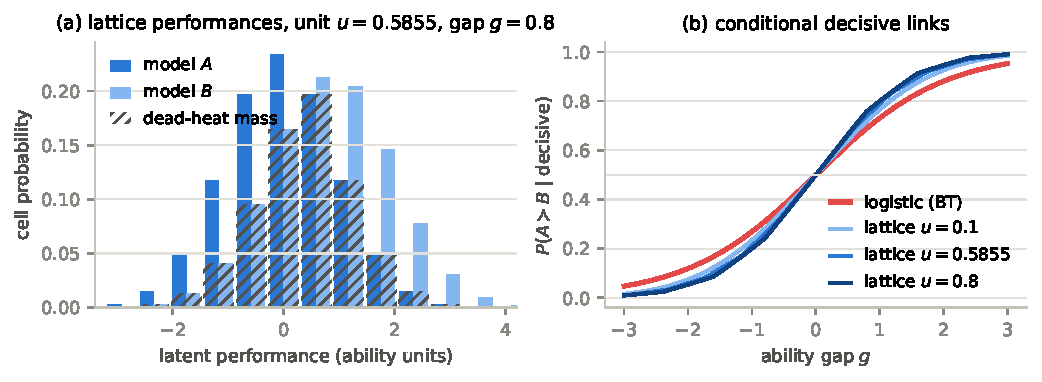
\includegraphics[width=\linewidth]{figures/fig_model.pdf}
\caption{The lattice gap-link model. \textbf{(a)} Discretized
performance distributions at gap $g=0.8$, width $u=0.5855$ (a coarse
$L=12$ lattice is drawn so cells are visible; fits use $L=500$).
Hatched: dead-heat mass---both performances in the same cell.
\textbf{(b)} Conditional decisive links, Eq.~\eqref{eq:fdec}. Lattice
links are steeper than the logistic at the origin (slopes
$0.290$--$0.337$ vs.\ $0.25$) and steepen as the tie band widens.}
\label{fig:model}
\end{figure}

\subsection{The lattice family: ties as dead heat, steepness as a
side effect}

Following \citet{cotton2021}, discretize the noise onto a lattice of
cell width $u$. Performances land on cells $x_j = ju$; with
$a_j(g) = \Pr(X_A = x_j)$ and $b_j = \Pr(X_B = x_j)$,
\begin{equation}\label{eq:lattice}
W(g) = \sum_j a_j(g)\,\Pr(X_B < x_j), \qquad
D(g) = \sum_j a_j(g)\, b_j, \qquad
L(g) = W(-g).
\end{equation}
A tie is a dead heat: both draws in one cell
(Figure~\ref{fig:model}a). The width $u$ is the single tie parameter,
fit by profile likelihood. The induced decisive link is
\begin{equation}\label{eq:fdec}
F_u(g) = \frac{W(g)}{W(g)+L(g)}.
\end{equation}
Two facts organize everything downstream. First, $F_u$ is steeper than
the logistic at a toss-up---$F_u'(0)$ is $0.290$, $0.324$, $0.337$ at
$u \in \{0.1, 0.5855, 0.8\}$ against $\sigma'(0)=0.25$---and steepens
as $u$ grows. Carving dead-heat mass from the middle of the distribution
sharpens what remains; the logistic's slope is unattainable at any
width. Second, as a consequence, one parameter controls tie mass
\emph{and} decisive steepness. The family cannot move one without the
other. We call this \emph{entanglement} and measure its price in
Section~\ref{sec:rq4}.

\subsection{Davidson: ties by extension, orthogonal by theorem}

\citet{davidson1970} extends BT with a tie outcome. In gap form, with
$\nu \geq 0$ and $Z_\nu(g) = 2\cosh(g/2) + \nu$,
\begin{equation}\label{eq:davidson}
\Pr(A \succ B \mid g) = \frac{e^{g/2}}{Z_\nu(g)}, \qquad
\Pr(\text{tie} \mid g) = \frac{\nu}{Z_\nu(g)}, \qquad
\Pr(B \succ A \mid g) = \frac{e^{-g/2}}{Z_\nu(g)}.
\end{equation}

\begin{theorem}[Tie orthogonality]\label{thm:orth}
For every $\nu \geq 0$, Davidson's conditional decisive link is exactly
logistic: $\Pr(A \succ B \mid \mathrm{decisive}, g) = \sigma(g)$.
\end{theorem}

\begin{proof}
Conditioning on a decisive outcome cancels $Z_\nu$:
$e^{g/2}/(e^{g/2}+e^{-g/2}) = \sigma(g)$.
\end{proof}

Theorem~\ref{thm:orth} makes the two families a perfectly matched pair.
Each has one ability per model and one tie parameter. They differ in
exactly one structural respect: Davidson's tie parameter never touches
its decisive link, and the lattice's always does. Every tie-related
question in this paper comes back to this theorem---including why a
decisive-only comparison of BT and Davidson would be vacuous, and what
the both-bad stress test of Section~\ref{sec:rq4} is actually measuring.

\subsection{Estimation and conventions}

All fits are per-vote maximum likelihood with analytic gradients; only
the link differs between methods. Where an experiment replicates the
production leaderboard's outcome treatment, decisive votes count twice
in their direction and each tie once in each direction through the
decisive link (\emph{half-tie} mode); where tie prediction is itself the
question, the full trinomial $\{W,D,L\}$ likelihood is used. All fits of
all methods anchor the same reference model
(\texttt{gpt-4-0613}~$=0$: a dated checkpoint, present with high volume
in every training window; the production anchor enters too late for our
earliest refits). Cross-link ability magnitudes are rescaled by
$F'(0)/0.25$ so a reported unit buys the same win-probability change at
a toss-up---the analogue of BT's $400/\ln 10$ Elo constant---and are
labeled convention-dependent. Sign conventions for calibration deltas
are stated once per results section.

% ==================================================================
\section{How much could the link matter? Effect ceilings}
\label{sec:ceiling}

The question ``is this link better?'' has a computable prerequisite:
``how much better could \emph{any} link be?'' Both links are fit to the
same votes and scored on the same outcomes, so if one family were
exactly true, the other's best-fitting member would concede at most a
computable amount---an amount that depends only on the two link shapes
and on where the data put their ability gaps. With $\hat P$ the
vote-weighted empirical distribution of fitted gaps and $F_u$ a lattice
truth, the logistic's minimal concession is
\begin{equation}\label{eq:ceiling}
C = \min_{s>0}\ \mathbb{E}_{g\sim\hat P}\,
\mathrm{KL}\!\left(\mathrm{Bern}(F_u(g)) \,\big\|\,
\mathrm{Bern}(\sigma(g/s))\right).
\end{equation}
Real matchups concentrate near toss-ups---the median fitted $|g|$ is
$0.31$---exactly where all increasing links agree. Evaluated across
every plausible width and skew, Eq.~\eqref{eq:ceiling} gives
$C \leq 0.23\times$MPD, where MPD is the pre-registered minimum
practical difference of Section~\ref{sec:data}; the trinomial analogue
for tie mechanisms is $\leq 0.31\times$MPD in \emph{both} truth
directions. Since per-model flexibility absorbs still more, these are
upper bounds.

Three consequences. First, the honest a-priori expectation for every
calibration comparison in this paper was practical equivalence---we
recorded that expectation before fitting, and any verdict exceeding a
ceiling would itself have demanded a misspecification investigation.
Second, the ceiling is falsifiable by a second route that involves no
held-out scoring at all: every gap link makes the overidentifying
triple prediction
$F^{-1}(p_{AC}) = F^{-1}(p_{AB}) + F^{-1}(p_{BC})$, so if the links are
interchangeable on real gaps, their triple residuals must be
indistinguishable too. Section~\ref{sec:rq2b} confirms this
independently. Third, the methodology travels: for any two candidate
models of the same data, an hour of arithmetic on the empirical design
distribution can reveal---before any experiment---that the comparison
cannot practically matter. We offer the ceiling as a reusable
pre-analysis step, and this paper as a case study in what happens when
it is taken seriously.

% ==================================================================
\section{Data and pre-registered protocol}\label{sec:data}

\paragraph{Data.} The largest public Arena battle log: $1{,}799{,}991$
anonymous pairwise battles, $129$ models, sub-second timestamps,
2023-04-24 to 2024-08-14; the platform's deduplication retains
$1{,}670{,}250$, which all fits use. Outcomes are \{A wins, B wins, tie,
tie (both bad)\}. Quality ties are $20.45\%$ of non--both-bad votes over
the full period, up from $13.1\%$ in the first three months---a drift
that recurs throughout. The replication set is the 2025 release:
$135{,}634$ battles, $53$ models, fourteen weeks
(Section~\ref{sec:repl}).

\paragraph{Pipeline validation.} Refitting BT at the published
leaderboard's own timestamp reproduces the published ratings to MAE
$0.18$ Elo points (Spearman $0.99997$, all $128$ models). Across ten
published BT-era snapshots the era-appropriate variant achieves MAE
$0.18$--$1.01$ on nine of ten; the tenth (2024-04-03) is an unexplained
outlier at $2.26$, reported rather than dropped.

\paragraph{Thresholds.} Statistical significance is free at
$n \approx 10^6$, so verdicts use a derived \emph{minimum practical
difference}. For decisive calibration: a uniform $10$-Elo-point gap
error ($\epsilon = 10\ln 10/400$ nats) costs
$\tfrac12 p(1-p)\epsilon^2 = 4.1\times10^{-4}$ at a toss-up, so
$\text{MPD}_3 = 4\times10^{-4}$ nats/vote. For trinomial tie
calibration: a one-point error in $\Pr(\text{tie})$ at the observed
$\sim\!20\%$ level gives $\text{MPD}_4 = 3\times10^{-4}$. Sub-MPD
effects are practically equivalent regardless of significance.

\paragraph{Gates and verdicts.} The full pipeline passed synthetic
ground-truth gates before real data: correct-sign detection at true
effects down to $0.3\times$MPD, correct positive calls at $\geq$MPD,
no false positives in sub-MPD worlds, tie-parameter recovery within
$10\%$. One gate finding matters later: under high parameter noise, a
\emph{correctly specified} steep link loses held-out to misspecified BT
($-1.41\times$MPD)---plugin predictions from steep links are
overconfident; bootstrap-calibrated standard errors (Fisher deflated by
the measured $0.80$; $\rho = 0.983$ against the published bootstrap)
showed this reversal is inactive at our pooled noise levels. Verdicts
come from a fixed classifier over thirteen rolling monthly windows
(cumulative training, next-month testing): \emph{positive} needs
$|\bar\Delta| \geq \text{MPD}$, ten-of-thirteen sign consistency, and a
window-cluster bootstrap CI (effective $N = 13$, always stated)
excluding zero; \emph{equivalence} needs the CI inside
$(-\text{MPD},+\text{MPD})$, with significant sub-MPD leans reported as
leans, never wins; anything else is \emph{inconclusive}. Post-hoc
analyses are labeled and never override a pre-registered verdict.
Machinery ablations (labeled) confirm the apparatus is not doing the
work: pooled CIs move by under $0.004\times$MPD across bootstrap sizes
$10^3$--$5\times10^4$; link curves are invariant to lattice resolution
(to $10^{-15}$ in the half-width, $3\times10^{-4}$ in the gap grid, with
full-population refits identical to five decimals); and the profiled tie
width moves by under $0.6\%$ across profile-grid densities.
Models absent from training are unscoreable and counted:
$24.8$--$75.8\%$ of decisive test votes per window, a deployment fact
in its own right.

% ==================================================================
\section{Results}\label{sec:results}

\subsection{Stability: rankings do not move differently}\label{sec:rq1}

When new models enter and the leaderboard refits, whose incumbent
rankings move less? For each adjacent checkpoint pair we fit both
methods on identical cumulative data and compare incumbent rankings
($\geq 1000$ votes; an all-models variant matches throughout).

\begin{figure}[t]
\centering
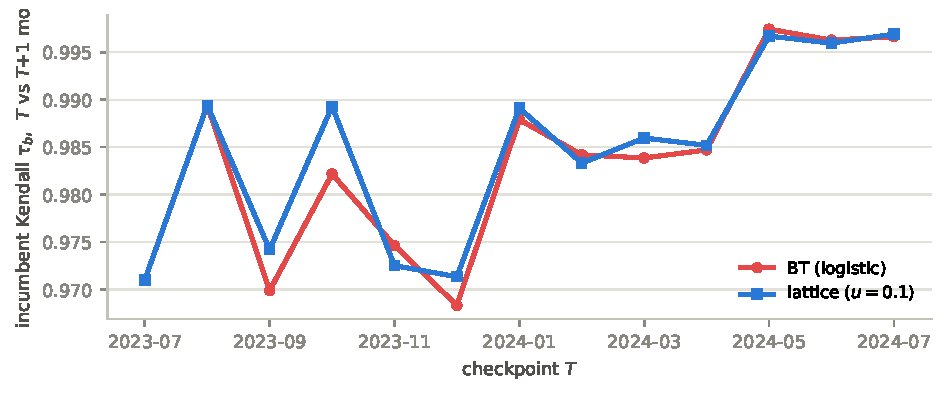
\includegraphics[width=\linewidth]{figures/fig_rq1.pdf}
\caption{Month-over-month incumbent ranking stability (Kendall
$\tau_b$) for BT and the lattice link. The curves are statistically
indistinguishable---median paired difference $+0.00026$---while both
improve together as the pool matures. Source:
\texttt{rq1\_metrics.csv}.}
\label{fig:rq1}
\end{figure}

The answer is a null with nothing hiding in it. Median paired
$\tau_b$ difference $+0.00026$; the lattice better in $7$ windows, worse
in $4$, tied in $2$; means $0.98469$ versus $0.98358$; the largest
single-window difference is $0.00713$. The same picture holds at all
three lattice widths, both horizons, both incumbent sets. No incumbent
moved more than five rank positions in any window under either method,
and slope-matched ability drift is $1.70$--$1.77$ Elo-equivalent points
per month for every method. Meanwhile stability itself varies from
$\tau_b = 0.968$ to $0.997$ across windows as the pool matures---roughly
two orders of magnitude more than any between-method difference. The
operative lever is sample size, not link family. A labeled post-hoc
check found no modulation by entrant count or entrant vote share (all
$|\rho| \leq 0.37$, $n=13$).

Rankings do not move differently. Section~\ref{sec:ceiling} predicted
why: where the data live, these links barely differ. That prediction
can be tested directly, with no fitting at all.

\subsection{Link shape: the ceiling, confirmed without fitting}
\label{sec:rq2b}

Every gap link must satisfy triple additivity. For each of $786$ dense
stable triples (legs $\geq 100$ decisive votes inside 60-day blocks,
members present throughout), the standardized residual
\begin{equation}\label{eq:zstat}
z = \frac{F^{-1}(\hat p_{AC}) - F^{-1}(\hat p_{AB}) -
F^{-1}(\hat p_{BC})}{\sqrt{v_{AB}+v_{BC}+v_{AC}}},
\qquad
v_{XY} = \frac{\hat p(1-\hat p)}{n_{XY}\,[F'(F^{-1}(\hat p))]^2},
\end{equation}
should be standard normal if the link shape is right and preferences
are stable. Mean $z^2$ measures shape misfit scale-invariantly, so the
links compete fairly.

\begin{figure}[t]
\centering
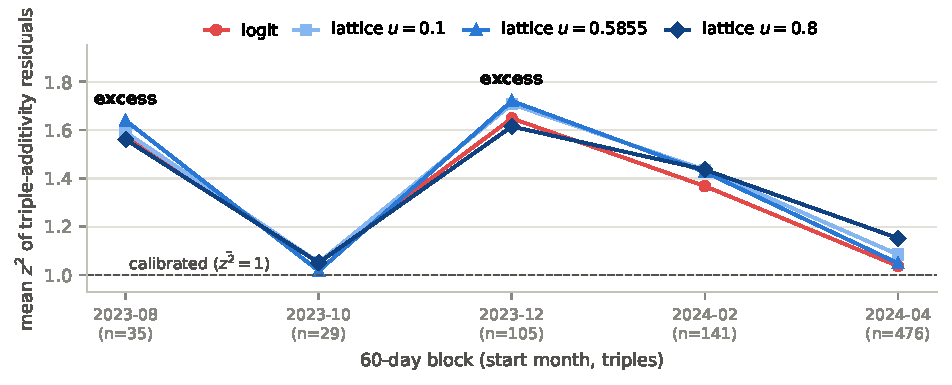
\includegraphics[width=\linewidth]{figures/fig_rq2b.pdf}
\caption{Mean squared triple-additivity residual per 60-day block, per
link. The four links are inseparable---their spread matches the test's
synthetically measured no-power band---while two blocks show a shared
excess no link explains (Section~\ref{sec:anomaly}). Source:
\texttt{rq2b\_blocks.csv}.}
\label{fig:rq2b}
\end{figure}

Pooled mean $z^2$: logit $1.202$; lattice $1.231$, $1.252$, $1.279$
across widths. Synthetic calibration passed (true-link $z^2 =
1.02$--$1.03$) and showed the statistic cannot separate these links at
real gap scales: in both generating directions the four links differ by
$0.01$--$0.04$, the same order as the real spread. This is the effect
ceiling of Eq.~\eqref{eq:ceiling} re-derived by an entirely different
instrument---within-window ranking consistency, no held-out scoring, no
plugin estimates, no time splits---and it reaches the same verdict:
\emph{at the gaps real matchups occupy, no member of this family is
distinguishable from the logistic.} Two structurally different tests
agreeing is stronger than either alone.

Shape is settled. But calibration on \emph{future} votes could still
differ: estimation noise interacts with steepness even when shapes
agree in-sample. That is the next question.

\subsection{Calibration: equivalent --- and a cautionary tale}
\label{sec:rq3}

Both methods are fit per window in half-tie mode and scored by log loss
on the shared scoreable decisive votes of the following month. Sign
convention: $\Delta = \ell\ell_{\text{BT}} - \ell\ell_{\text{lattice}}$;
positive favors the lattice.

\begin{figure}[t]
\centering
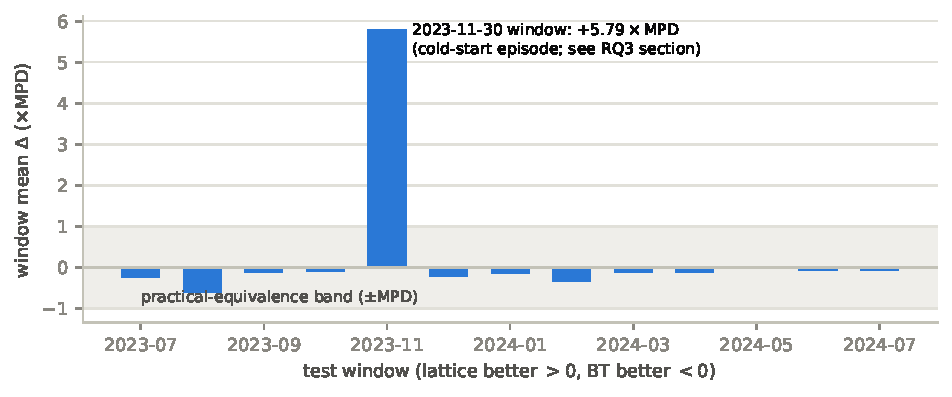
\includegraphics[width=\linewidth]{figures/fig_rq3.pdf}
\caption{Per-window calibration delta (primary width $u=0.5855$), in
MPD units. Every window of thirteen lies inside the
practical-equivalence band. Source:
\texttt{rq3\_window\_table\_u0.5855.csv}.}
\label{fig:rq3}
\end{figure}

\textbf{Verdict: equivalence, with a sub-practical BT-leaning lean, at
all three widths.} Pooled $-0.121\times$MPD, CI $(-0.191, -0.074)$ at
the primary width; $-0.148$ $(-0.201,-0.116)$ and $-0.226$
$(-0.321,-0.164)$ at the others; BT better in $12$--$13$ of $13$
windows; \emph{every} window inside the band
(Figure~\ref{fig:rq3}; largest $0.63\times$MPD). The lean is real and
below deployment relevance---per protocol it is reported as a lean,
not a win. It is largest at the steepest width but not monotone across
the two shallower ones: directional, qualified evidence for the
plugin-overconfidence mechanism of Section~\ref{sec:data}. The
pre-registered strata agree. Recent-entrant votes: $-0.110\times$MPD,
CI $(-0.172, -0.052)$. And in the one location where the pre-analysis
said a lattice-truth effect could clear MPD---the early high-noise
recent-entrant stratum, predicted $+1.58\times$MPD under
lattice-truth---the measurement is $-0.275\times$MPD, CI
$(-1.169, +0.040)$: the prediction is excluded decisively.

Two shared measurements dwarf all of this. Reliability slopes on
held-out predictions are $1.46$ for every method: everything is
underconfident on next month's votes by the same factor, a
nonstationarity no link addresses---and uncertainty-integrated
(posterior-predictive-style) prediction does not help, shifting the
pooled delta only from $-0.121$ to $-0.117\times$MPD and reliability to
$1.46$ (labeled post-hoc; Gauss--Hermite over calibrated standard
errors). Coverage is worse: up to three quarters of next-month decisive
votes involve an unscoreable newcomer. Drift and coverage bind;
the link does not.

\subsubsection{The episode that wasn't}\label{sec:artifact}

Our first run of this experiment told a better story, and it was wrong.
It returned \emph{inconclusive}: twelve sub-practical windows plus one
at $+5.8\times$MPD, traced to a single model that entered with two
training votes, which BT extrapolated to mid-table
($\hat\theta = +0.43$) while the steeper lattice held near zero. We
initially read this as implicit shrinkage---a steep link regularizing
cold starts. A reviewer-driven follow-up asked whether explicit ridge
regularization could reproduce the effect, and its $\lambda \approx 0$
baseline refused to match our own stored table. The audit that followed
found the cause: our earlier lattice implementation paired
piecewise-linear log-likelihood values with smoothed gradients, and
that inconsistency---originally noticed only as an optimizer
nuisance---had effectively clamped near-zero-data models in the curve
tails. With consistent interpolation the episode vanishes
(old code $+5.792\times$MPD, corrected $+0.017$, byte-identical
everything else; the corrected lattice places the cold-start model at
$+0.29$, barely below BT's $+0.38$), the unfiltered result equals the
old cold-start-filtered one, and the verdict above is what remains.
All synthetic gates were re-certified under the corrected code.

The retraction sharpened the science. \emph{Steepness is not implicit
regularization}---but explicit regularization works exactly as the
false story promised: ridge on BT shrinks the cold-start model's
estimate from $+0.38$ to $0.00$ over $\lambda \in [1,3]$ and improves
that window by ${\sim}5.5\times$MPD, while established models move by
at most $0.015$. Cold-start protection is real, cheap, and
link-independent. And the episode is a working demonstration of the
protocol: pre-registered baselines plus one skeptical follow-up caught
an artifact that a lone headline run would have published.

Calibration, then, cannot separate the families. By
Theorem~\ref{thm:orth}, ties are the one outcome channel where they
differ by construction. Is that difference measurable?

\subsection{Ties: provably different shapes, indistinguishable fit ---
and the price of entanglement}\label{sec:rq4}

Both models are fit per window by trinomial likelihood---abilities plus
one profiled tie parameter each---and scored on next month's
\{win, loss, tie\} outcomes. Dead heats use the platform's quality-tie
label; ``both bad'' marks responses below an absolute bar, not close
draws, and enters only the stress test below. Sign convention:
$\Delta = \ell\ell_{\text{Davidson}} - \ell\ell_{\text{lattice}}$;
positive favors the lattice; $\text{MPD}_4 = 3\times10^{-4}$.

\textbf{Verdict: inconclusive, by one episode.} Pooled
$+0.838\times$MPD, CI $(+0.017, +2.542)$; lattice better in $10/13$
windows, but the estimate is carried by a single window at
$+9.55\times$MPD. Decomposition attributes that window to the tie
channel on near-peer, largely same-family pairs (tie votes $+407$ nats
versus $-301$ decisive; sibling matchups such as
\texttt{gpt-4-0314} vs.\ \texttt{gpt-4-1106-preview} lead), where the
window's tie rate ran high and the lattice's tie-curve shape briefly
paid off. A cold-start filter does not touch it ($+0.861\times$MPD):
this episode, unlike Section~\ref{sec:artifact}'s, is real data
behaving unusually for one month---it immediately precedes one of the
two anomaly eras of Section~\ref{sec:anomaly}, a coincidence we note
without claiming.

\begin{figure}[t]
\centering
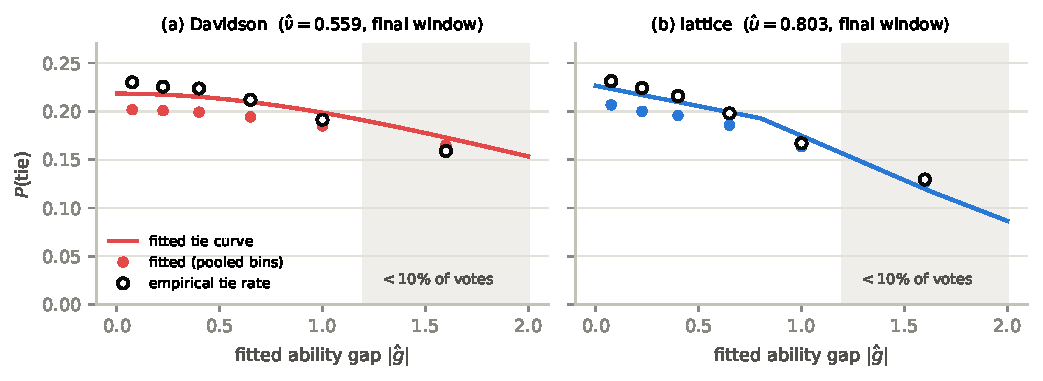
\includegraphics[width=\linewidth]{figures/fig_rq4_curves.pdf}
\caption{Fitted tie curves versus empirical tie rates, pooled with vote
weights, each model binned by its own fitted gaps. The mechanisms agree
at the origin, decay at structurally different rates, and the region
where they separate (shaded) carries under $10\%$ of votes. Source:
\texttt{rq4\_tie\_curve\_bins.csv}.}
\label{fig:rq4curves}
\end{figure}

\textbf{Different shapes the data cannot discriminate.} The fitted
mechanisms imply nearly identical at-zero tie mass in every window
(within ${\sim}0.01$) but structurally different bands: the tie
probability halves at $2.84$--$2.93$ ability units under Davidson's
slow decay versus $1.67$--$1.68$ under the lattice's overlap decay---a
stable $1.7\times$ difference. Held-out fit cannot pick a side
(vote-weighted binned RMS $0.0225$ vs $0.0237$), because real matchups
concentrate where the shapes agree (Figure~\ref{fig:rq4curves}). The
parameters $\nu$ and $u$ carry genuinely different shape content---they
are not relabelings---but this dataset cannot say which shape is right.
That is a more precise statement than ``equivalent,'' and we intend the
distinction.

\begin{figure}[t]
\centering
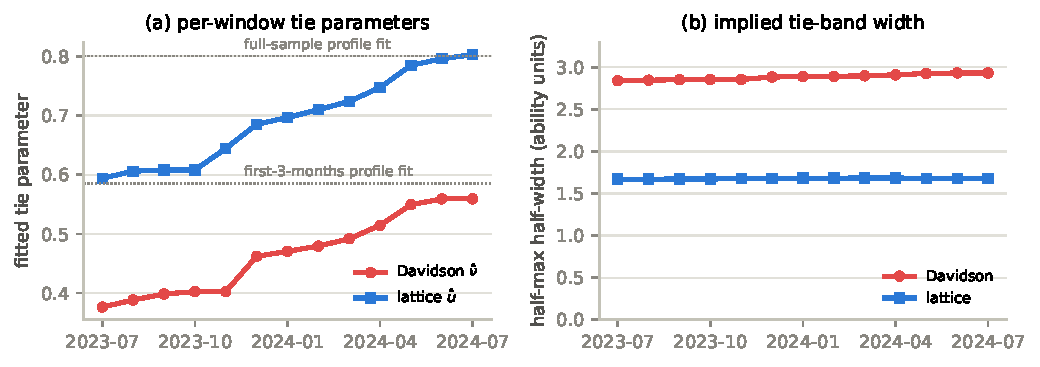
\includegraphics[width=\linewidth]{figures/fig_rq4_traj.pdf}
\caption{Drift trajectories. \textbf{(a)} Per-window profiled tie
parameters rise together ($\hat\nu\!: 0.376 \to 0.559$;
$\hat u\!: 0.594 \to 0.803$), tracking the tie-share drift
($13.1\% \to 20.45\%$); the endpoints independently reproduce two
earlier one-shot profile fits (dotted). \textbf{(b)} The implied
band-width difference is stable throughout. Source:
\texttt{rq4\_param\_trajectories.csv}.}
\label{fig:rq4traj}
\end{figure}

\textbf{Drift, cross-validated three ways.} Both tie parameters rise
near-monotonically across the sixteen months
(Figure~\ref{fig:rq4traj}), tracking the raw tie-share drift; any
single pooled tie parameter averages a moving target, which is why
every experiment profiles per window. The windowed trajectory's
endpoints reproduce, to ${\sim}0.01$, two estimates computed
independently by a different procedure months earlier---three
estimation paths agreeing on one drifting quantity.

\textbf{The price of entanglement, measured.} Theorem~\ref{thm:orth}
says Davidson's $\nu$ cannot touch its decisive link; the lattice's $u$
must. Forcing both models to absorb both-bad-scale tie mass
(${\sim}35\%$ of votes) makes this concrete: the lattice width pins at
its pre-specified profile ceiling in $11/13$ windows---not for want of
tie capacity but because its narrow band must over-widen to cover
large-gap ties---and on identical held-out \emph{decisive} votes its
log loss degrades by $+4.75\times$MPD (ceiling-window mean) versus
$+2.50$ for the Davidson control, which isolates the shared
ability-refit effect since its decisive link provably cannot move. The
lattice-specific excess, ${\approx}2.2\times$MPD, is the measured cost
of buying tie mass with decisive accuracy. Qualifications: modest,
window-heterogeneous, and the profile boundary was never stress-tested
at this tie scale; the tie/both-bad category decision rests on its
conceptual grounds, not on this result.

\subsection{Replication: a second dataset}\label{sec:repl}

Every design above, transported verbatim to the 2025 Arena release
($135{,}634$ battles, $53$ models, twelve weekly windows; labeled
post-hoc generalization since the transport itself was not
pre-registered): full-population fits agree at Spearman $0.999839$ with
a maximum rank move of one; the calibration comparison returns
equivalence with the same sub-practical BT lean at all three widths
($-0.084$/$-0.175$/$-0.176\times$MPD; BT better in $11/12$ windows);
the tie comparison is again lattice-leaning inconclusive
($+0.779\times$MPD, CI $(+0.382, +1.093)$); and the profiled width
barely moves over fourteen weeks ($0.689 \to 0.693$), confirming the
tie-propensity drift as a long-horizon phenomenon. Same nulls, same
lean directions, same structural picture, different era and pool.

% ==================================================================
\section{The anomaly: excess dispersion no link explains}
\label{sec:anomaly}

One signal in this dataset survives every attribution attempt, and we
promote it deliberately: in two specific eras, \emph{every} link we
tested fails triple additivity the same way. Blocks
2023-08-22$\to$10-21 and 2023-12-20$\to$2024-02-18 show mean
$z^2 = 1.57$ and $1.65$, with $13$--$14\%$ of triples beyond $|z|>2$
against a nominal $4.6\%$; other blocks sit near calibration. Half-block
splits localize the first episode to roughly late September--October
2023 and show the second persisting undiminished in both halves, so
within-window drift is not the mechanism. Ruled out systematically: the
platform's deduplication transition (overlaps only the cleanest block);
entry activity (the excess blocks have \emph{fewer} entries and lower
entrant vote share---anti-correlated); language mix, judge counts,
votes per judge, tie share, duplicated-prompt share (none separates
excess from clean); single-model artifacts (excess triples span models
near base rates). Because the excess is invariant across link shapes,
it is a property of the vote-generating process itself.

Two candidate explanations remain live. \emph{Judge-population
composition shifts}: a mixture of individually consistent judges
violates additivity in aggregate. \emph{Genuine context effects}: votes
influenced by what else occupies the pool---the classical IIA-violation
mechanism, appearing here as a shared failure of every IIA-\emph{like}
model rather than a differential one. Distinguishing them needs
per-judge panel structure or listwise data that public releases do not
provide. We had pre-registered an entry-proximity event study for
exactly this purpose and descoped it on evidence: the excess is
anti-correlated with entries, so an entry-based instrument is
structurally wrong for it. We state the anomaly as an open question,
and as a concrete data request to preference platforms.

% ==================================================================
\section{Discussion}\label{sec:discussion}

\begin{figure}[t]
\centering
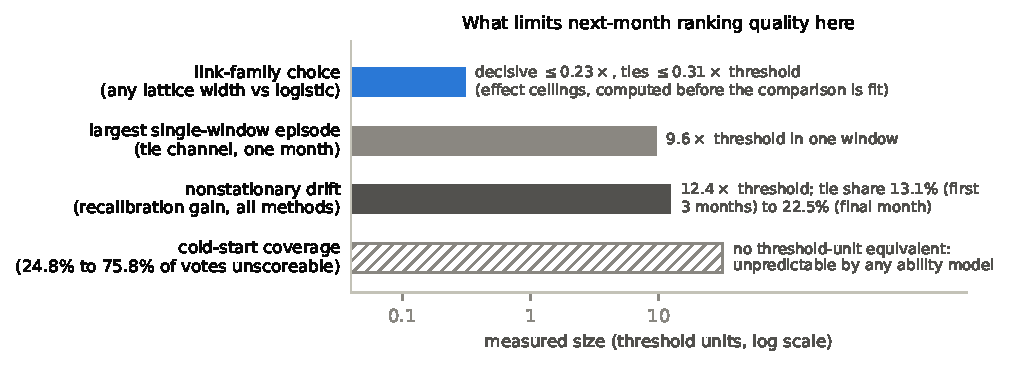
\includegraphics[width=\linewidth]{figures/fig_concept.pdf}
\caption{The error budget of this deployment, schematically. Link
choice is bounded above by construction; episodes, shared drift, and
cold-start coverage each exceed it by one to two orders of magnitude in
their own terms. Annotated values are measured; bar lengths are not to
scale.}
\label{fig:concept}
\end{figure}

\paragraph{The general principle.} Every result above is one theme
instantiated: richer links buy approximation accuracy, and this system's
errors are not approximation errors. Figure~\ref{fig:concept} draws the
budget. The quantity a link controls is bounded at a fraction of one
practical unit by Eq.~\eqref{eq:ceiling}; everything that actually
limits ranking quality---shared drift miscalibration ($1.46\times$
underconfidence for every method), cold-start coverage (up to
three-quarters of votes unscoreable), single-month episodes (up to
${\sim}10\times$MPD)---lives on other axes entirely. The statistical
lesson travels beyond leaderboards. Reward models for RLHF are BT by
construction, and listwise or richer-link refinements of the preference
objective~\citep{liu2024lipo} face the same arithmetic: where comparison
data concentrates near toss-ups and the candidate pool churns,
estimation error, drift, and coverage dominate any link-shape
refinement. Recommendation and matchmaking systems consuming implicit
pairwise feedback, and econometric choice models fit to large
observational panels, inherit the same check-list: compute the ceiling
before the comparison. Expressiveness is the right investment only when
approximation error is the binding constraint, and in evolving
preference systems it rarely is.

\paragraph{What to do instead.} The audit's constructive findings are
an ordered to-do list for platform operators. First, cold starts:
explicit ridge (or any shrinkage prior) on new entrants buys the
protection that no link provides, at ${\sim}5\times$MPD in the one
month our data offered a natural experiment, with negligible effect on
established models. Second, drift: recalibrate predictions against
recent outcomes---posterior-predictive smoothing of parameter
uncertainty does not substitute, because the miscalibration is shared
drift, not plugin overconfidence. Third, ties: if ties matter to the
product, prefer mechanisms that are orthogonal by construction
(Theorem~\ref{thm:orth}); a single-width dead-heat band pays for tie
mass with decisive accuracy. Only after all that, consider the link.

\paragraph{On negative results.} The pre-registration protocol was not
ornamental. The ceilings set expectations before fitting; the gates
certified detection power; the fixed classifier refused convenient
readings twice; and the discipline caught our own numerical artifact
when one skeptical baseline refused to reproduce a stored table
(Section~\ref{sec:artifact}). We offer the protocol as the reason these
nulls are informative rather than disappointing, and the artifact
episode as the argument for auditing positive stories with the same
energy as negative ones.

% ==================================================================
\section{Limitations}\label{sec:limits}

This paper is not a test of \citet{cotton2021}'s multi-entrant
coherence theorem; pairwise data cannot exercise it. Conclusions
concern one platform (two eras of it) and the gap-link families
compared; TrueSkill-style approximate Bayesian inference was positioned
but not tested. The ridge demonstration rests on one natural
experiment. The dose-response evidence for plugin overconfidence is
directional, not monotone. The entanglement measurement is qualified by
its untested profile boundary. One validation snapshot remains an
unexplained outlier. And the anomaly of Section~\ref{sec:anomaly} is
characterized but not explained---resolving it, like testing field
coherence, needs data that platforms do not currently release: judge
panel structure and listwise comparisons.

% ==================================================================
\section{Conclusion}

We asked whether a better-motivated choice model improves a real
preference leaderboard, and built the audit carefully enough to trust
the answer: no---and provably, almost no such improvement was
available. One theorem, one ceiling, four pre-registered comparisons,
one replication, one retracted episode, and one open anomaly later, the
durable lesson is the one we began with. \emph{Richer models help when
approximation error dominates estimation error.} In large, noisy,
evolving preference systems---leaderboards, reward models,
recommenders---estimation error, nonstationarity, and cold starts
overwhelm the link function. Spend expressiveness where the errors are.

\bibliography{refs}

\end{document}
